\documentclass[handout,aspectratio=169]{beamer}
\usetheme{default}

\usepackage{geometry}
\usepackage{amsthm}
\usepackage{xcolor}
\usepackage{mathtools}
\usepackage{amsfonts}
\usepackage{multicol}
\usepackage{graphicx} % Allows including images
\usepackage{booktabs} % Allows the use of \toprule, \midrule and \bottomrule in tables
\usepackage{tikz,pgfplots}
\tikzset{>=latex}
\usetikzlibrary{arrows,automata,shapes,calc,matrix}
\definecolor{bgTUE}{HTML}{f1efef}
\definecolor{fgTUE}{HTML}{000000}
%----------------------------------------------------------------------------------------
%	TITLE PAGE
%----------------------------------------------------------------------------------------

\title{Verifying SPLs using parity games expressing variability} % The short title appears at the bottom of every slide, the full title is only on the title page

\institute[TU/e] % Your institution as it will appear on the bottom of every slide, may be shorthand to save space
{
	\begin{columns}
\begin{column}{0.5\textwidth}
	\begin{center}
	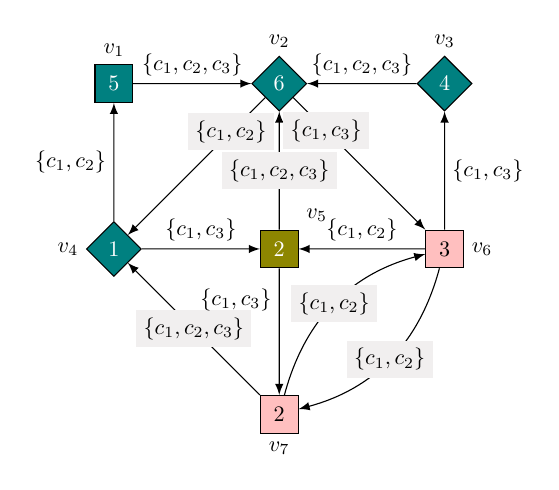
\begin{tikzpicture}[->,scale=0.7, every node/.style={scale=0.8}]
	\tikzstyle{even} = [diamond,draw,minimum size=0.75cm]
	\tikzstyle{odd}  = [rectangle,draw,shape aspect=1,minimum size=0.6cm]
	
	\node[odd, label=north:$v_1$,fill=teal,text=white] (v1) at (20,20) {5};
	\node[even,label=north:$v_2$,fill=teal,text=white] (v2) at (23,20) {6};
	\node[even,label=north:$v_3$,fill=teal,text=white] (v3) at (26,20) {4};
	
	\node[even,label=west:$v_4$,fill=teal,text=white]  (v4) at (20,17) {1};
	\node[odd, label=north east:$v_5$,fill=olive,text=white] (v5) at (23,17) {2};
	\node[odd, label=east:$v_6$,fill=pink] (v6) at (26,17) {3};
	
	\node[odd, label=south:$v_7$,fill=pink] (v7) at (23,14) {2};
	
	
	\path (v1) edge node[above]{$\{c_1,c_2,c_3\}$} (v2);
	\path (v3) edge node[above]{$\{c_1,c_2,c_3\}$} (v2);
	
	\path (v4) edge node[left]{$\{c_1,c_2\}$} (v1);
	\path (v2) edge node[fill=bgTUE,near start]{$\{c_1,c_2\}$} (v4);
	\path (v4) edge node[above]{$\{c_1,c_3\}$} (v5);
	\path (v5) edge node[fill=bgTUE]{$\{c_1,c_2,c_3\}$} (v2);
	\path (v6) edge node[above]{$\{c_1,c_2\}$} (v5);
	\path (v2) edge node[fill=bgTUE,near start]{$\{c_1,c_3\}$} (v6);
	\path (v6) edge node[right]{$\{c_1,c_3\}$} (v3);
	
	
	\path (v7) edge node[fill=bgTUE]{$\{c_1,c_2,c_3\}$} (v4);
	\path (v5) edge node[left,near start]{$\{c_1,c_3\}$} (v7);
	\path (v7) edge[bend left] node[fill=bgTUE]{$\{c_1,c_2\}$} (v6);
	\path (v6) edge[bend left] node[fill=bgTUE]{$\{c_1,c_2\}$} (v7);
	\end{tikzpicture}
\end{center}
\end{column}
	\begin{column}{0.5\textwidth}
		\begin{center}
			\large
			Sjef van Loo\\
			\medskip\small
			6 November, 2019\\
			\bigskip
			\bigskip
			\bigskip
			\bigskip
			\bigskip
			\bigskip
\textit{Msc Thesis \\
Computer Science and Engineering\\
\medskip
Supervised by T.A.C. Willemse}\\
\end{center}
\end{column}
\end{columns}
}
\date{November 6, 2019} % Date, can be changed to a custom date
\setbeamertemplate{footline}[frame number]
\begin{document}
	\setbeamercolor{footline}{bg=white}
\setbeamercolor{normal text}{fg=fgTUE,bg=bgTUE}\usebeamercolor*{normal text}
\setbeamercolor{title}{fg=fgTUE}
\setbeamercolor{subtitle}{fg=fgTUE}
\setbeamercolor{titlelike}{fg=fgTUE}
\setbeamercolor{alerted text}{fg=fgTUE}
\setbeamercolor{example text}{fg=fgTUE}

%\setbeamercolor{structure}{fg=fgTUE}

\setbeamercolor{background canvas}{parent=normal text}
%\setbeamercolor{background}{parent=background canvas}

\setbeamercolor{palette primary}{fg=fgTUE,bg=bgTUE} % changed this
\setbeamercolor{palette secondary}{use=structure,fg=fgTUE} % changed this
\setbeamercolor{palette tertiary}{use=structure,fg=fgTUE} % changed this
\setbeamercolor{box1}{fg=fgTUE,bg=white}
\setbeamercolor{itemize item}{fg=fgTUE,bg=white}
\setbeamercolor{itemize subitem}{fg=fgTUE,bg=white}
\setbeamercolor{itemize subsubitem}{fg=fgTUE,bg=white}
\setbeamercolor{enumerate item}{fg=fgTUE,bg=white}
\setbeamercolor{enumerate subitem}{fg=fgTUE,bg=white}
\setbeamercolor{enumerate subsubitem}{fg=fgTUE,bg=white}
\setbeamertemplate{footline}{
	{%
		\leavevmode%
		\hbox{%
			\begin{beamercolorbox}[wd=.1\paperwidth,ht=3ex,dp=1ex,right]{box1}%
				\insertframenumber
			\end{beamercolorbox}%
			\begin{beamercolorbox}[wd=0.05\paperwidth,ht=3ex,dp=1ex,left]{box1}%
			\end{beamercolorbox}%
			\begin{beamercolorbox}[wd=0.7\paperwidth,ht=3ex,dp=1ex,left]{box1}%
				\inserttitle
			\end{beamercolorbox}%
			\begin{beamercolorbox}[wd=0.12\paperwidth,ht=3ex,dp=1ex,right]{box1}%
				
\includegraphics[height=3ex]{TUE}
			\end{beamercolorbox}%
			\begin{beamercolorbox}[wd=0.03\paperwidth,ht=3ex,dp=1ex,right]{box1}%
			\end{beamercolorbox}}%
}}

\begin{frame}
\titlepage % Print the title page as the first slide
\end{frame}
%----------------------------------------------------------------------------------------
%	PRESENTATION SLIDES
%----------------------------------------------------------------------------------------

\begin{frame}[t]
\frametitle{Outline}
\begin{columns}[t]
	\begin{column}{0.5\textwidth}
		\begin{itemize}
			\item Verification \& SPLs
			\item Problem statement
			\item Variability Parity Games
			\item VPG algorithms
			\item Experimental results
		\end{itemize}
	\end{column}
	\begin{column}{0.5\textwidth}
	\end{column}
\end{columns}
\end{frame}

%------------------------------------------------

\begin{frame}[t]
\frametitle{Verification \& SPLs}
\begin{columns}[t]
	\begin{column}{0.5\textwidth}
		\begin{itemize}
			\item Formally verify software by modelling its behaviour and expressing a requirement
			\item SPLs describe multiple software products, it does so by using features
			\item TODO: LTS en FTS uitleggen? Wellicht noemen maar niet uitleggen...
		\end{itemize}
	\end{column}
	\begin{column}{0.5\textwidth}
	\end{column}
\end{columns}
\end{frame}
%------------------------------------------------

\begin{frame}[t]
\frametitle{Problem statement}
\begin{columns}[t]
\begin{column}{0.5\textwidth}
	\begin{itemize}
		\item Verify all the products in an SPL
		\item Do so more efficiently than verifying them independently
	\end{itemize}
\end{column}
\begin{column}{0.5\textwidth}
\end{column}
\end{columns}
\end{frame}

%----------------------------------------------------------------------------------------

\begin{frame}[t]
\frametitle{Variability parity game}
\begin{columns}[t]
	\begin{column}{0.5\textwidth}
		\begin{itemize}
			\item Explain Parity Games using an example
			\item What does solving a PG mean
			\item PGs can be used to check software products
		\end{itemize}
	\end{column}
	\begin{column}{0.5\textwidth}
		\begin{itemize}
			\item Explain VPGs using an example
			\item What does solving a VPG mean
			\item VPGs can be used to check SPLs
		\end{itemize}
	\end{column}
\end{columns}
\end{frame}
%----------------------------------------------------------------------------------------

\begin{frame}[t]
\frametitle{VPG algorithms - Recursive algorithm}
\begin{columns}[t]
	\begin{column}{0.5\textwidth}
		\begin{itemize}
			\item The recursive algorithm reasons about sets of vertices
			\item Attractor calculation example
		\end{itemize}
	\end{column}
	\begin{column}{0.5\textwidth}
		\begin{itemize}
			\item the recursive algorithm for VPGs reasons about sets of vertex configuration pairs
			\item Attractor calculation example on VPG
			\item Function-wise representation to efficiently perform attractor calcs
			\item Short explanation of symbolic representation
			\item Time complexities
		\end{itemize}
	\end{column}
\end{columns}
\end{frame}

%----------------------------------------------------------------------------------------

\begin{frame}[t]
\frametitle{VPG algorithms - Incremental pre-solve algorithm}
\begin{columns}[t]
	\begin{column}{0.5\textwidth}
		\begin{itemize}
			\item Introduce algorithm
			\item Introduce pessimistic PGs
			\item We need an alg to solve PGs using pre-solved vertices for efficiency
		\end{itemize}
	\end{column}
	\begin{column}{0.5\textwidth}
	\end{column}
\end{columns}
\end{frame}

%----------------------------------------------------------------------------------------

\begin{frame}[t]
\frametitle{VPG algorithms - Incremental pre-solve algorithm}
\begin{columns}[t]
	\begin{column}{0.5\textwidth}
		\begin{itemize}
			\item FPIte, show FP formula
			\item Show modified FP formula
			\item Explain the efficiency gained
		\end{itemize}
	\end{column}
	\begin{column}{0.5\textwidth}
		\begin{itemize}
			\item Very short explanation of a fixed-point
		\end{itemize}
	\end{column}
\end{columns}
\end{frame}

%----------------------------------------------------------------------------------------

\begin{frame}[t]
\frametitle{VPG algorithms - Local solving}
\begin{columns}[t]
	\begin{column}{0.5\textwidth}
		\begin{itemize}
			\item explain local solving
			\item introduced local algs for the novel VPG algs and existing PG algs.
		\end{itemize}
	\end{column}
	\begin{column}{0.5\textwidth}
	\end{column}
\end{columns}
\end{frame}

%----------------------------------------------------------------------------------------

\begin{frame}[t]
\frametitle{Experimental results - SPL games}
\def\scalegraphs{0.6}
\begin{columns}[t]
	\begin{column}{0.5\textwidth}
		\begin{figure}[H]
			\input{"../results/minepump/Zlnk product based_Zlnk fam based - explicit_Zlnk fam based - symbolic_"}
			\caption{Running times, in ms, on the minepump games.}
			\label{fig:results_minepump}
		\end{figure}%
	\end{column}
	\begin{column}{0.5\textwidth}
		\begin{figure}[H]
			\input{"../results/elevator/Zlnk product based_Zlnk fam based - explicit_Zlnk fam based - symbolic_"}
			\caption{Running times, in ms, on the elevator games.}
			\label{fig:results_elevator}
		\end{figure}%
	\end{column}
\end{columns}
\small
\raisebox{.7\height}{
\begin{tikzpicture}
\path[line width=2pt,color=cyan] (19,20) edge (20,20);
\end{tikzpicture}} Recursive algorithm for parity games\\
\raisebox{.7\height}{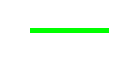
\begin{tikzpicture}
\path[line width=2pt,color=green] (19,20) edge (20,20);
\end{tikzpicture}} Recursive algorithm for VPGs with a symbolic representation of configurations\\
\raisebox{.7\height}{
\begin{tikzpicture}
\path[line width=2pt,color=red] (19,20) edge (20,20);
\end{tikzpicture}} Recursive algorithm for VPGs with an explicit representation of configurations\\
\end{frame}

%----------------------------------------------------------------------------------------

\begin{frame}[t]
\frametitle{Experimental results - SPL games}
\def\scalegraphs{0.6}
\begin{columns}[t]
	\begin{column}{0.5\textwidth}
		\begin{figure}[H]
			\input{"../results/minepump/Fixed-point product based_Incremental pre-solve_"}
			\caption{Running times, in ms, on the minepump games.}
			\label{fig:results_minepump}
		\end{figure}%
	\end{column}
	\begin{column}{0.5\textwidth}
		\begin{figure}[H]
			\input{"../results/elevator/Fixed-point product based_Incremental pre-solve_"}
			\caption{Running times, in ms, on the elevator games.}
			\label{fig:results_elevator}
		\end{figure}%
	\end{column}
\end{columns}
\small
\raisebox{.7\height}{
\begin{tikzpicture}
	\path[line width=2pt,color=violet] (19,20) edge (20,20);
	\end{tikzpicture}} Fixed-point iteration algorithm for parity games\\
\raisebox{.7\height}{
\begin{tikzpicture}
	\path[line width=2pt,color=orange] (19,20) edge (20,20);
	\end{tikzpicture}} Incremental pre-solve algorithm\\
\end{frame}

%----------------------------------------------------------------------------------------

\begin{frame}[t]
\frametitle{Experimental results - Random games}
\begin{columns}[t]
	\begin{column}{0.5\textwidth}
		\begin{itemize}
			\item Show the type of games where recursive symbolic fails and the explicit does not.
		\end{itemize}
	\end{column}
	\begin{column}{0.5\textwidth}
	\end{column}
\end{columns}
\end{frame}

%----------------------------------------------------------------------------------------

\begin{frame}[t]
\frametitle{Experimental results - Local solving}
\begin{columns}[t]
	\begin{column}{0.5\textwidth}
		\begin{itemize}
			\item Show the same graphs but with local solving as well
		\end{itemize}
	\end{column}
	\begin{column}{0.5\textwidth}
	\end{column}
\end{columns}
\end{frame}

%----------------------------------------------------------------------------------------

\begin{frame}[t]
\frametitle{Conclusions}
\begin{columns}[t]
	\begin{column}{0.5\textwidth}
		\begin{itemize}
			\item Collective approach can improve SPLs verifying performance
			\item The symbolic recursive can do this well
			\item The explicit recursive is "robust"
			\item Local solving can increase performance, however very dependent on alg \& type of VPG
		\end{itemize}
	\end{column}
	\begin{column}{0.5\textwidth}
	\end{column}
\end{columns}
\end{frame}

%----------------------------------------------------------------------------------------

\end{document}